% TeX'ing this file requires that you have AMS-LaTeX 2.0 installed
% as well as the rest of the prerequisites for REVTeX 4.0
%
% See the REVTeX 4 README file
% It also requires running BibTeX. The commands are as follows:
%
%  1)  latex apssamp.tex
%  2)  bibtex apssamp
%  3)  latex apssamp.tex
%  4)  latex apssamp.tex
%
\documentclass[prb,amsmath,amssymb, 10pt]{revtex4}
%\documentclass[preprint,showpacs,showkeys,preprintnumbers,amsmath,amssymb]{revtex4}

% Some other (several out of many) possibilities
%\documentclass[preprint,aps]{revtex4}
%\documentclass[aps, two column, amsmath,amssymb,floatfix]{revtex4}
%\documentclass[showkeys,showpacs,amsmath,amssymb,onecolumn,superscriptaddress,prl]{revtex4-1}% Physical Review B  
% \documentclass[aps,prl,reprint,showpacs,floatfix,superscriptaddress, onecolumn]{revtex4-2}

\usepackage{amsmath,amsthm,amssymb}
\usepackage{graphicx}% Include figure files
\usepackage{dcolumn}% Align table columns on decimal point
\usepackage{bm}% bold math
\usepackage{color}
\usepackage{epsfig}
\usepackage{multirow}
\usepackage{mathrsfs}
\usepackage{hyperref}
\usepackage{cleveref}
\usepackage{epstopdf}
\usepackage{subcaption}
\usepackage{autobreak}
\usepackage{tikz}
\usepackage{svg}
\usepackage{placeins}

%Macros for mathematical notations

\newcommand{\V}[1]{\boldsymbol{#1}} %# vector
\newcommand{\M}[1]{\boldsymbol{#1}} %# matrix
\newcommand{\Set}[1]{\mathbb{#1}} %# set
\newcommand{\D}[1]{\Delta#1} %# \D{t} for time step size
\renewcommand{\d}[1]{\delta#1} %# \d{t} for small increment
\newcommand{\norm}[1]{\left\Vert #1\right\Vert } % norm
\newcommand{\abs}[1]{\left|#1\right|} %abs

\newcommand{\grad}{\M{\nabla}} %gradient
\newcommand{\av}[1]{\left\langle #1\right\rangle } %take average

\newcommand{\sM}[1]{\M{\mathcal{#1}}} %matrix in mathcal font
\newcommand{\dprime}{\prime\prime} % double prime
%\global\long\def\i{\iota}
%\renewcommand{\i}{\iota} %i for imaginary unit
%\renewcommand{\i}{\mathsf i} %i for imaginary unit
\newcommand{\follows}{\quad\Rightarrow\quad} %=>
\newcommand{\eqd}{\overset{d}{=}} %=^d
\newcommand{\spe}[1]{\mathscr{#1}}  %important quantities in mathscr font
\newcommand{\eps}{\epsilon}
\newcommand{\bra}[1]{\left\langle #1 \right|}
\newcommand{\ket}[1]{\left| #1 \right\rangle}
\newcommand{\braket}[2]{\left\langle #1 \middle| #2 \right\rangle}
\newcommand{\bracket}[3]{\left\langle #1 \middle| #2 \middle| #3 \right\rangle}

\newtheorem{theorem}{Theorem}[section]
\newtheorem{lemma}[theorem]{Lemma}
\newtheorem{definition}[theorem]{Definition}



\begin{document}
\preprint{Preprint}

\title{Boundary integral method for Poisson's equation with orbital data}
\author{Xuanzhao Gao}
% \date{}

\maketitle

Currently, we have developed a boundary integral method to solve the Poisson's equation with dielectric interfaces using the orbital data as the source term.
In this note, I will briefly describe the solver, and show some preliminary results.

First, as been discussed in the previous notes, the equation to solve is given by
\begin{equation}\label{eq:sl_equation}
    \left( \frac{1}{2} \frac{\epsilon_i + \epsilon_j}{\epsilon_i - \epsilon_j} + D^T \right) \sigma(x) = - \partial_{\mathbf{n}} u_{\text{inc}}(x),~x \in \partial \Omega_i \cap \partial \Omega_j,
\end{equation}
where~$\sigma(x)$ is the unknown surface charge density,~$D^T$ is the transpose of the double layer potential operator, and~$u_{\text{inc}}(x)$ is the incident potential generated by the orbital data, given by
\begin{equation}
    \partial_{\mathbf{n}} u_{\text{inc}}(x) = \int_{\Omega_o} \frac{\partial G(x,y)}{\partial \mathbf{n}_x} \rho(y) dy.
\end{equation}
Eq.~\eqref{eq:sl_equation} is a Fredholm integral equation of the second kind~\cite{greengard1994numerical}, by solving which we can obtain the surface charge density~$\sigma(x)$, and then compute the potential and field at any point in the domain.
Our algorithm consists of the following steps to solve the above equation:
\begin{itemize}
    \item[1.] Load the orbital data and compute the charge density~$\rho(y)$ in the orbital region~$\Omega_o$
    \item[2.] Discretize the boundary into a set of panels, and evaluate $\partial_{\mathbf{n}} u_{\text{inc}}(x)$ on each panal
    \item[3.] Construct the discretized representation of the operator $\frac{1}{2} \frac{\epsilon_i + \epsilon_j}{\epsilon_i - \epsilon_j} + D^T$ using the discretized boundary
    \item[4.] Solve the resulting linear system to obtain the surface charge density $\sigma(x)$
\end{itemize}

We first load the wannier function stored in the \texttt{xsf} files.
For the ease of calculation, we shift the wannier function to be centered at the atom, and truncate the function in $z$ as shown below:
\begin{figure*}[htbp]
    \centering
    \begin{subfigure}[t]{0.3\textwidth}
        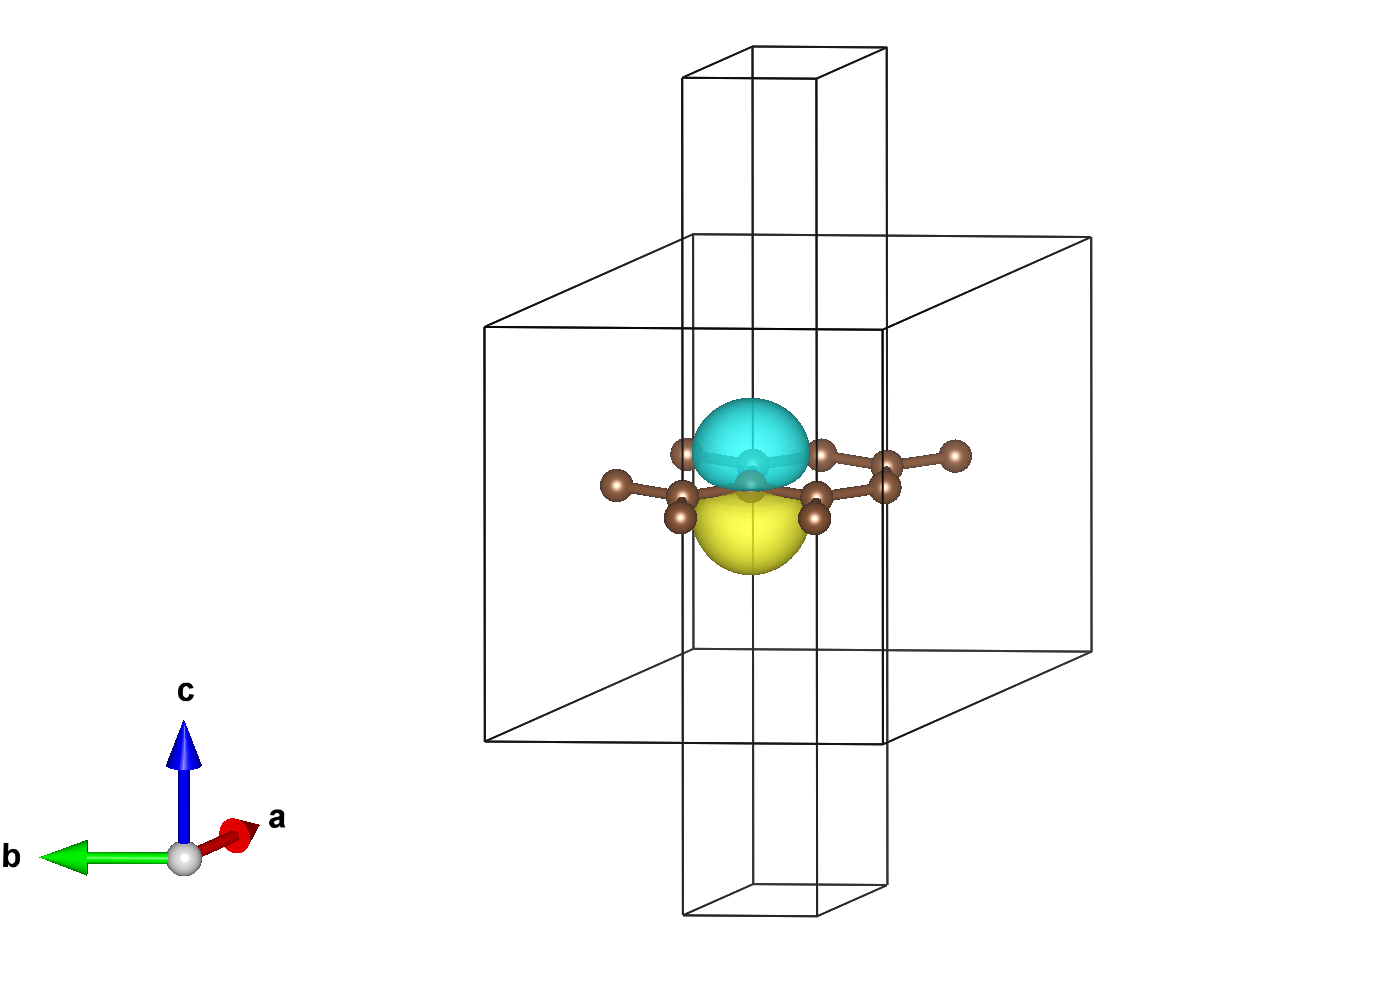
\includegraphics[width=\linewidth]{figs/oribital_data.png}
        \caption{\texttt{graphene\_00002\_shifted.xsf}}
    \end{subfigure}
    \begin{subfigure}[t]{0.3\textwidth}
        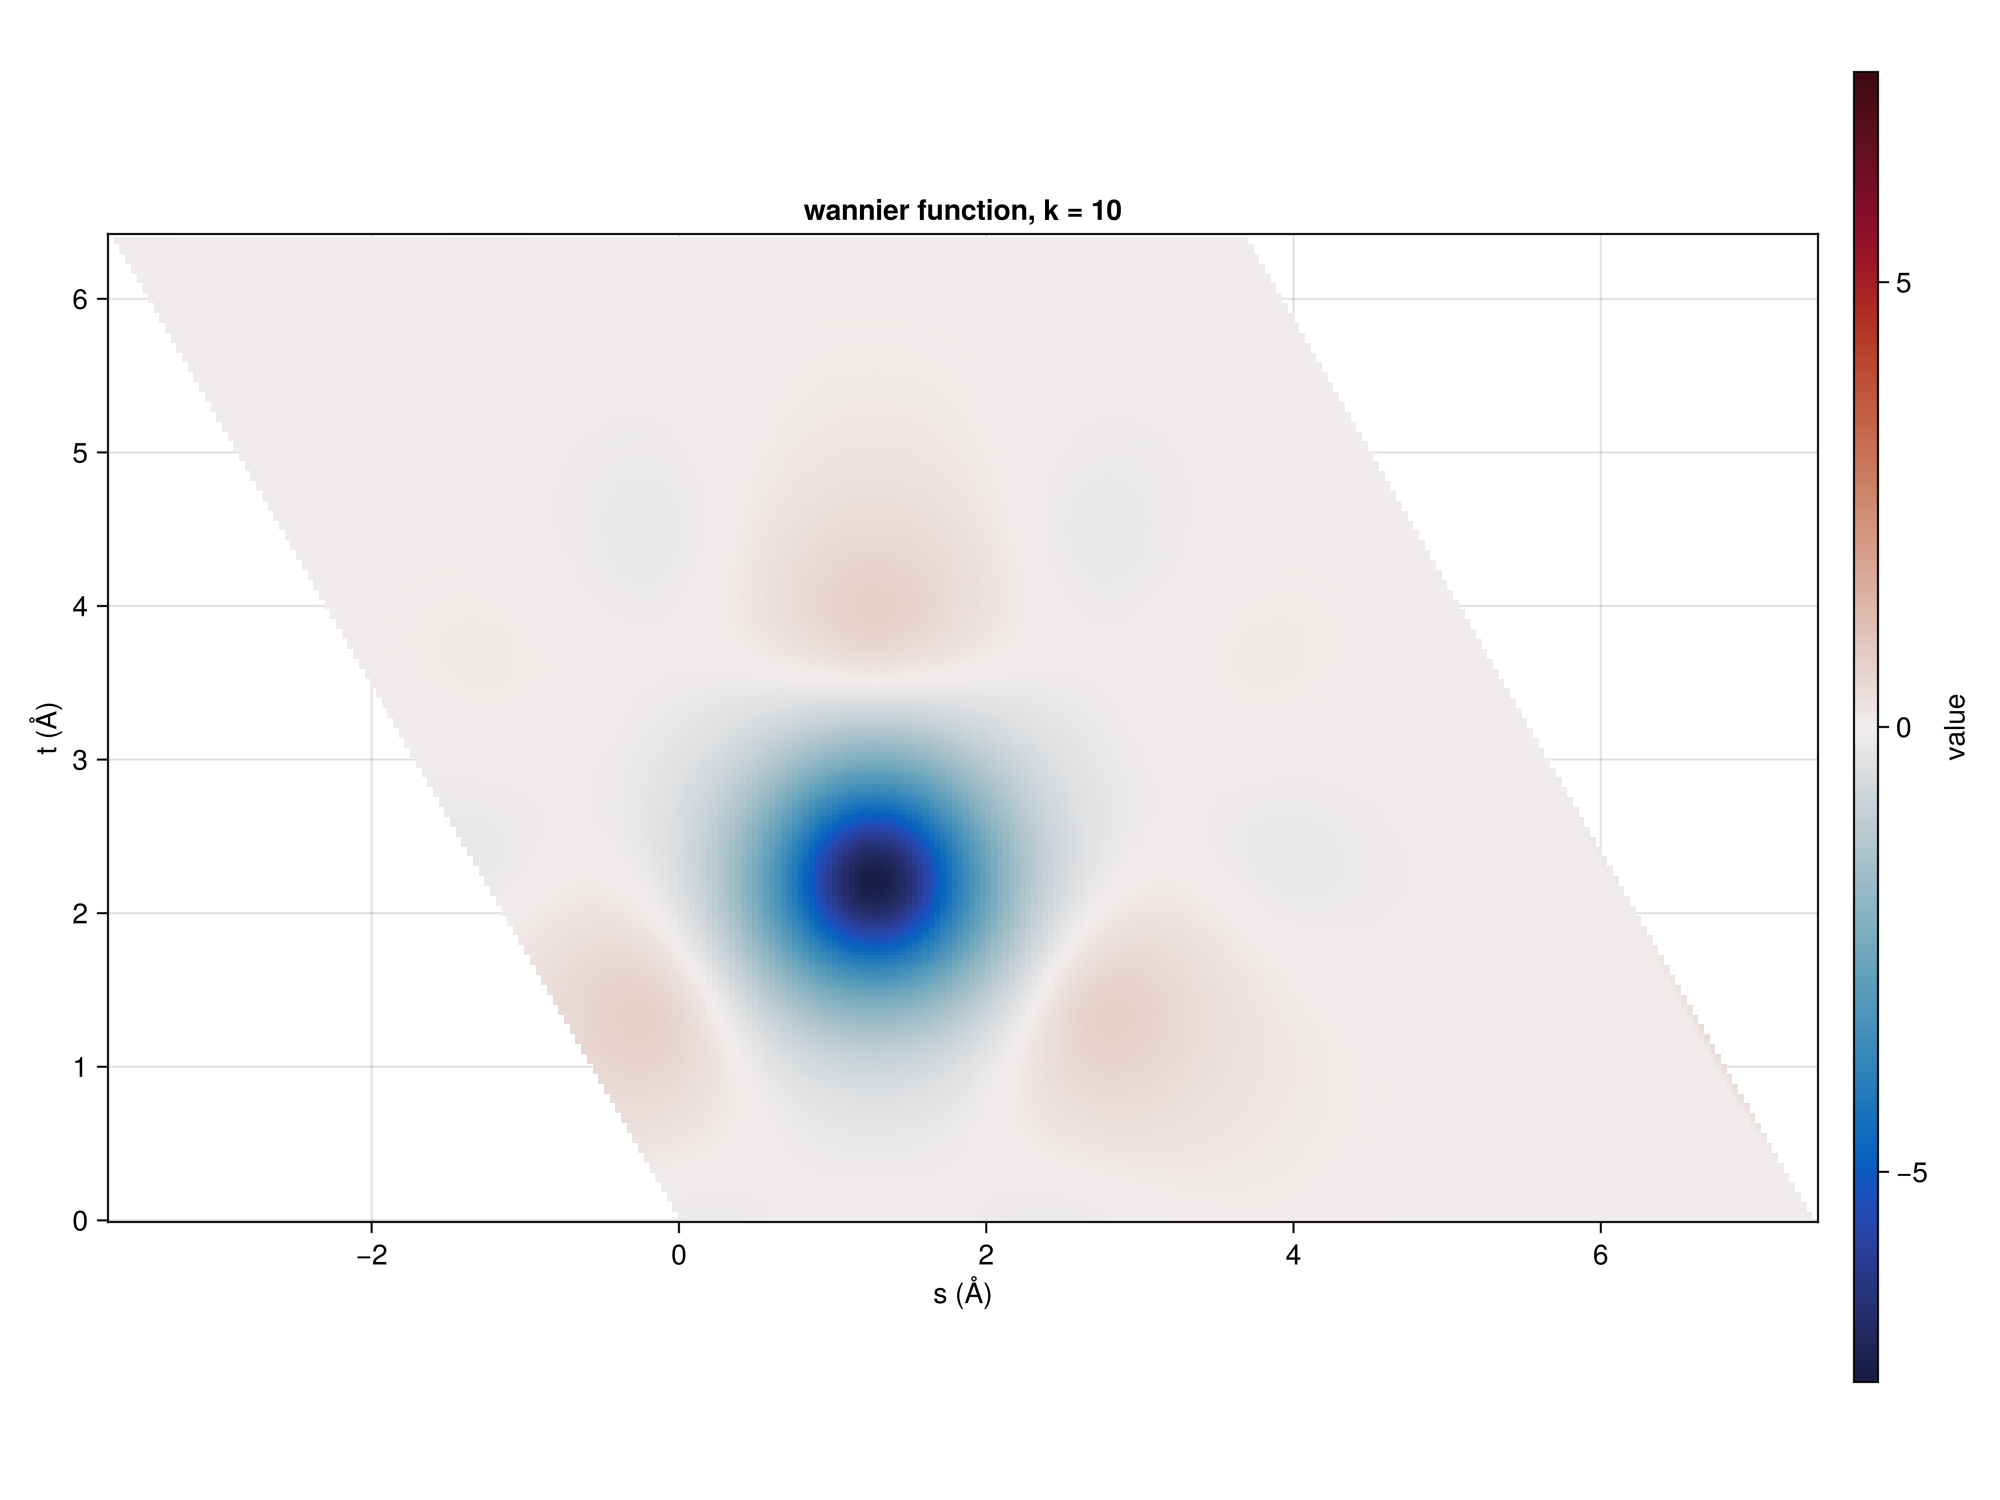
\includegraphics[width=\linewidth]{figs/graphene_00001_slice_k10.png}
        \caption{slice of \texttt{graphene\_00001.xsf}}
    \end{subfigure}
    \begin{subfigure}[t]{0.3\textwidth}
        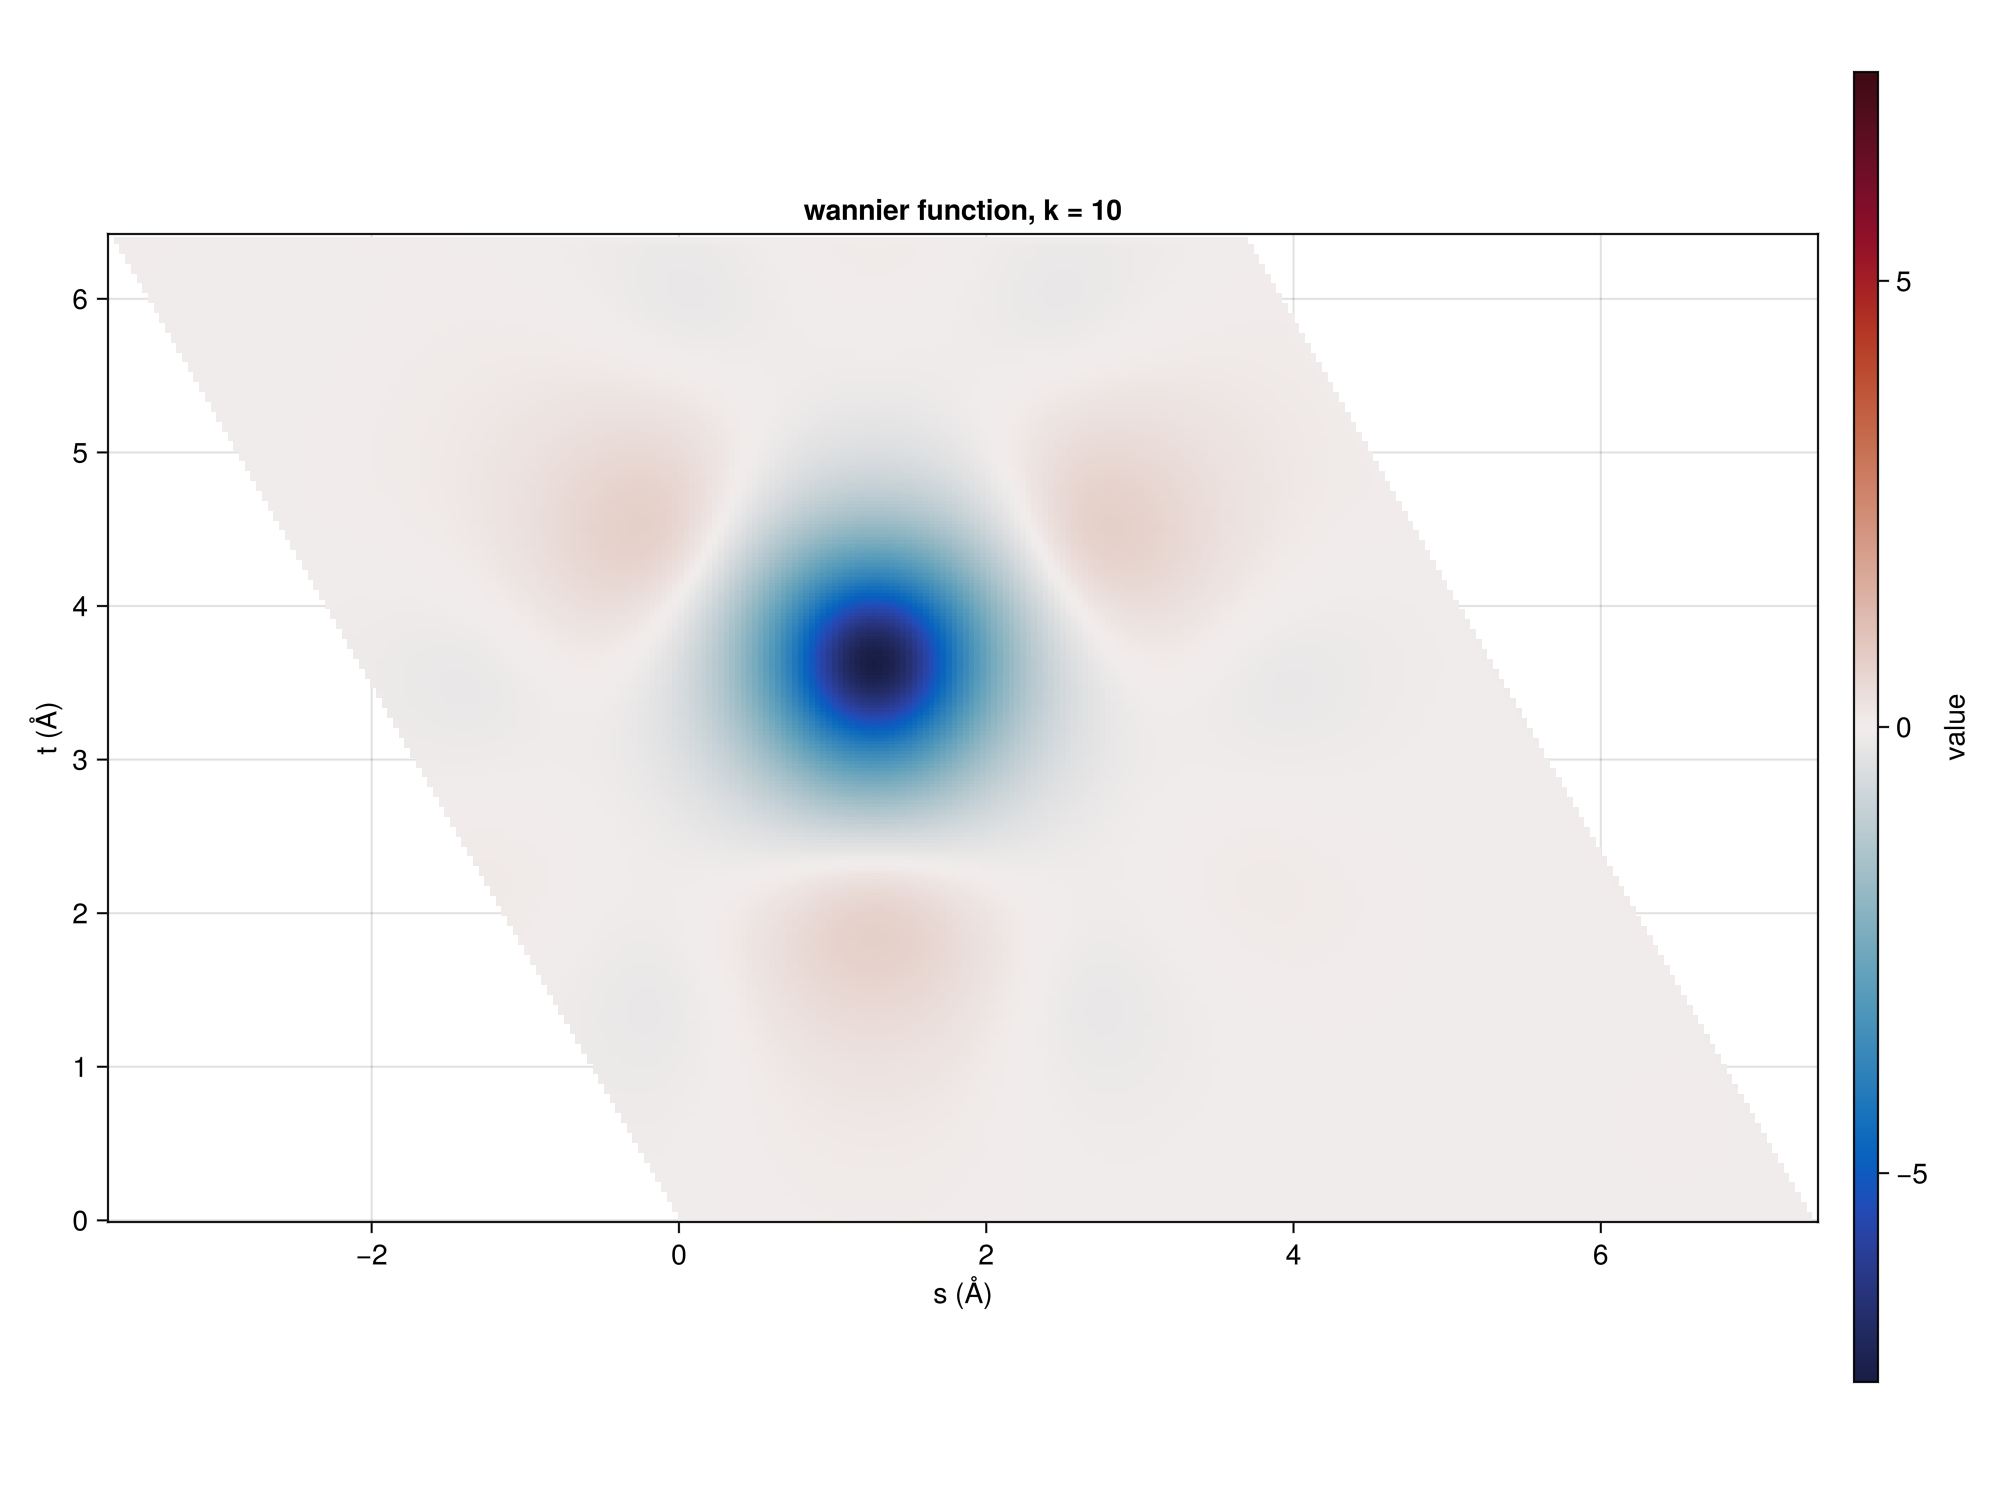
\includegraphics[width=\linewidth]{figs/graphene_00002_slice_k10.png}
        \caption{slice of \texttt{graphene\_00002.xsf}}
    \end{subfigure}
    \label{fig:wannier}
\end{figure*}

\FloatBarrier

Then by multiplying the wannier functions with each other, we can obtain the charge density $\rho(y)$. 
In the following examples, we simply consider the density by \texttt{graphene\_00002.xsf} with itself, which is inserted into a box of size $(90, 90, 9)$ to represent the 2D material, with relative permittivity $\epsilon_r = 6$.
Based on the charge density, we discretize the surface into panels, and on each panel we use a $p \times p$ Gauss-Legendre quadrature to sample the right hand side of Eq.~\eqref{eq:sl_equation}.
The orbital density and the panels are shown in Fig.~\ref{fig:panels}, where the panels near the orbital desity and edges are refined to capture the singularity of the kernel and the corner singularity, respectively.

\begin{figure}[htbp]
    \centering
    \begin{subfigure}[t]{0.4\textwidth}
        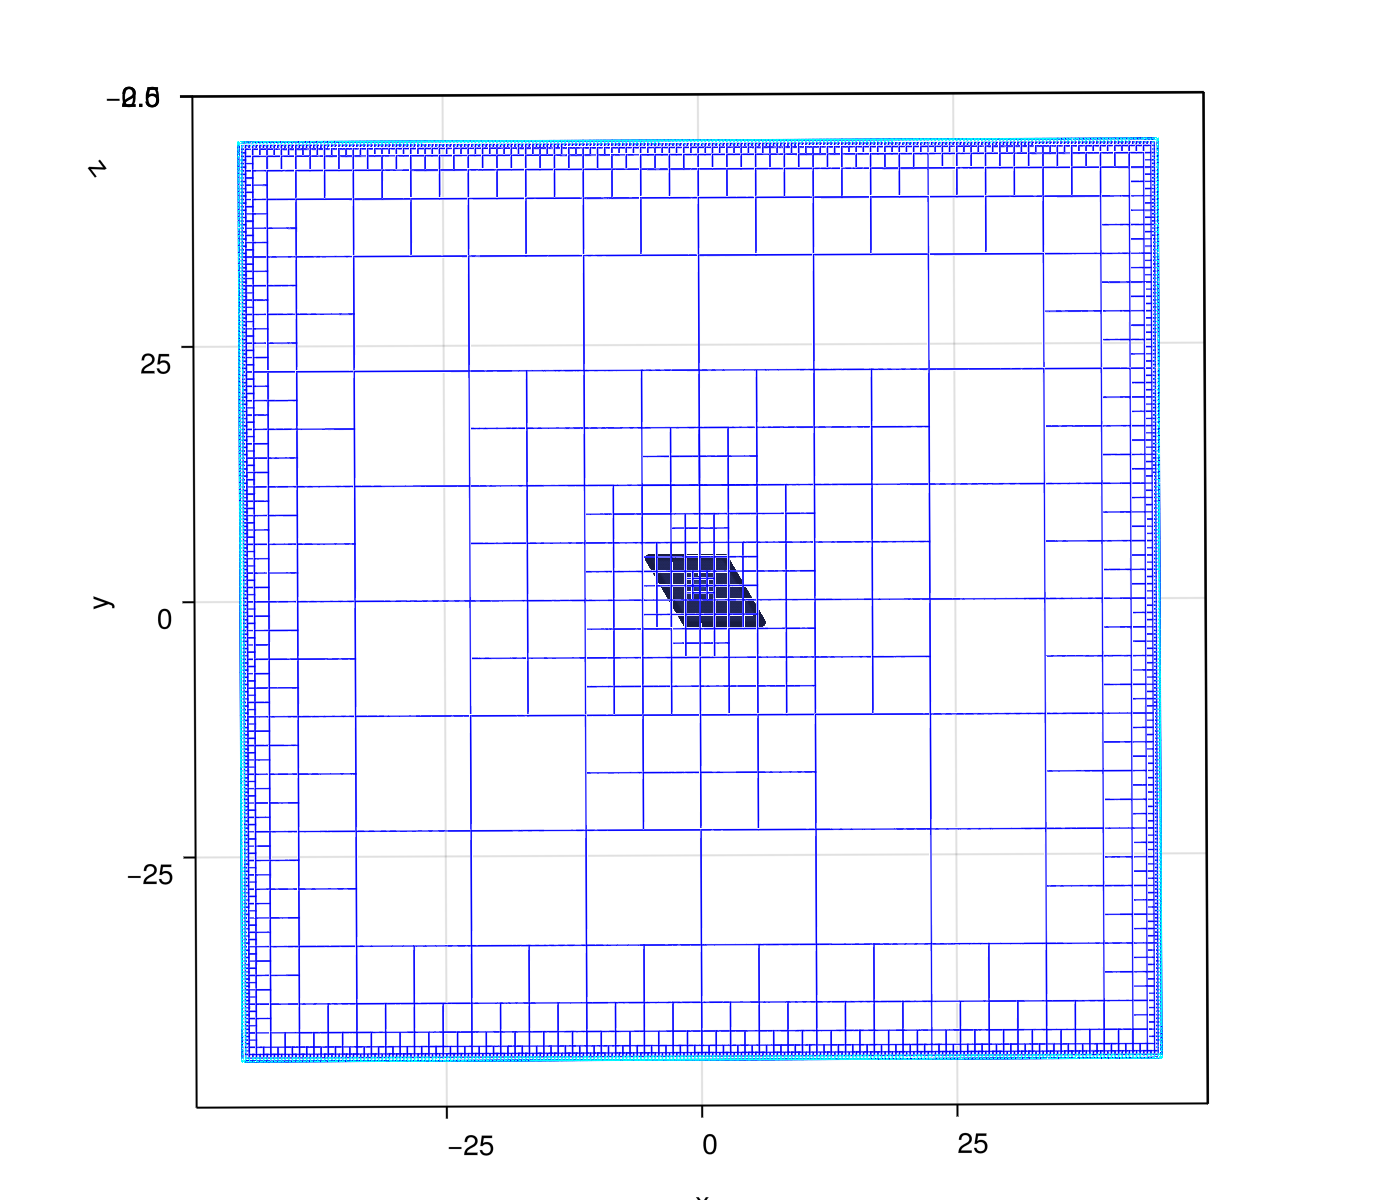
\includegraphics[width=\linewidth]{../codes/viz/figs/graphene_orbital_1.png}
    \end{subfigure}
    \begin{subfigure}[t]{0.4\textwidth}
        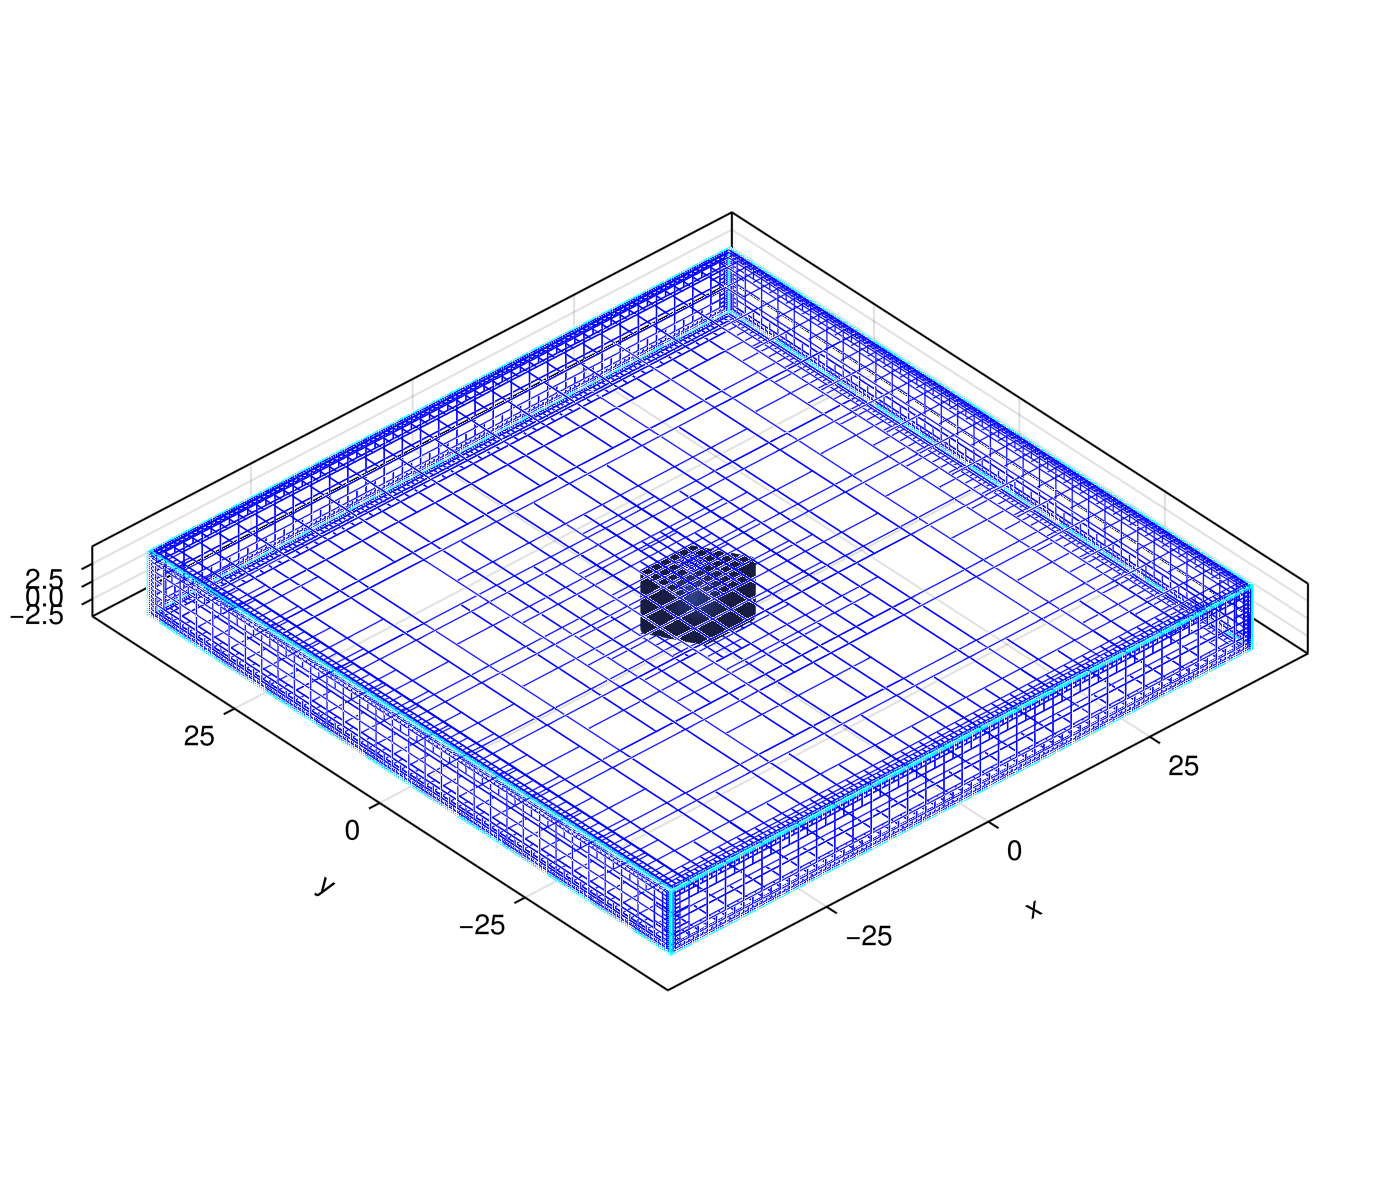
\includegraphics[width=\linewidth]{../codes/viz/figs/graphene_orbital_2.png}
    \end{subfigure}
    \caption{Orbital density and panels on the boundary of the dielectric interface.}
    \label{fig:panels}
\end{figure}

\FloatBarrier

With the discretized surface, we constructed a discretized representation of the operator/values on the left/right hand side of Eq.~\eqref{eq:sl_equation}, and solve the resulting linear system to obtain the surface charge density $\sigma(x)$, as shown in Fig.~\ref{fig:rhs_solution}.


\begin{figure}[htbp]
    \centering
    \begin{subfigure}[t]{0.4\textwidth}
        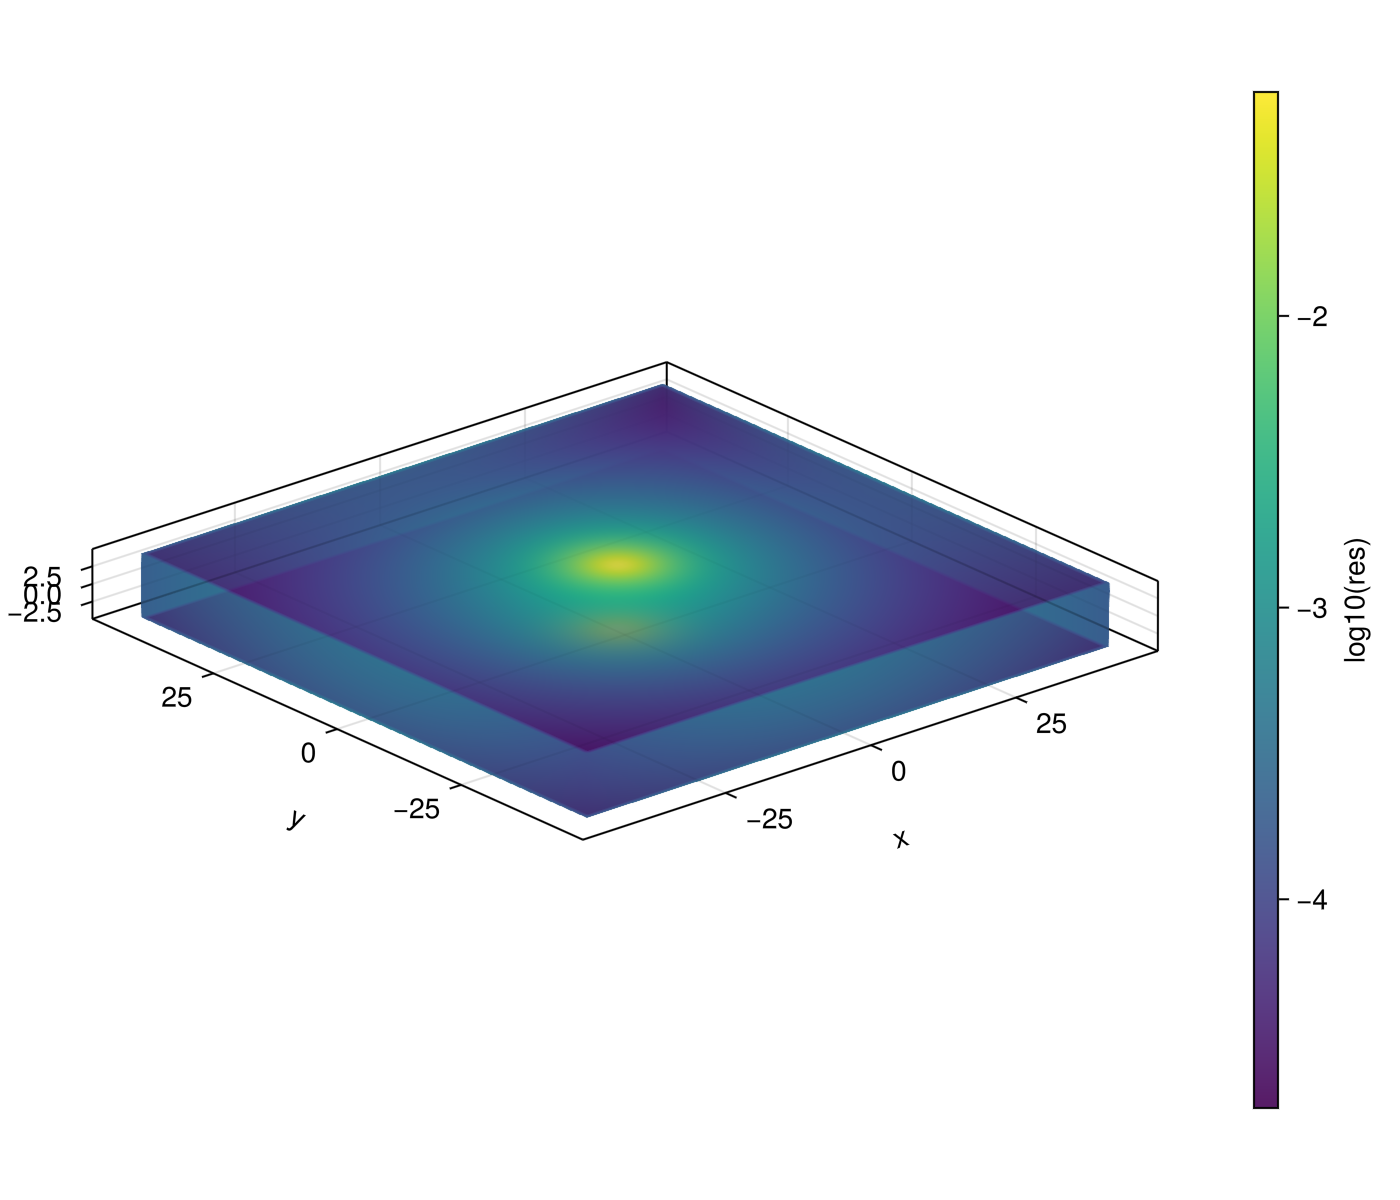
\includegraphics[width=\linewidth]{../codes/viz/figs/graphene_orbital_rhs.png}
    \end{subfigure}
    \begin{subfigure}[t]{0.4\textwidth}
        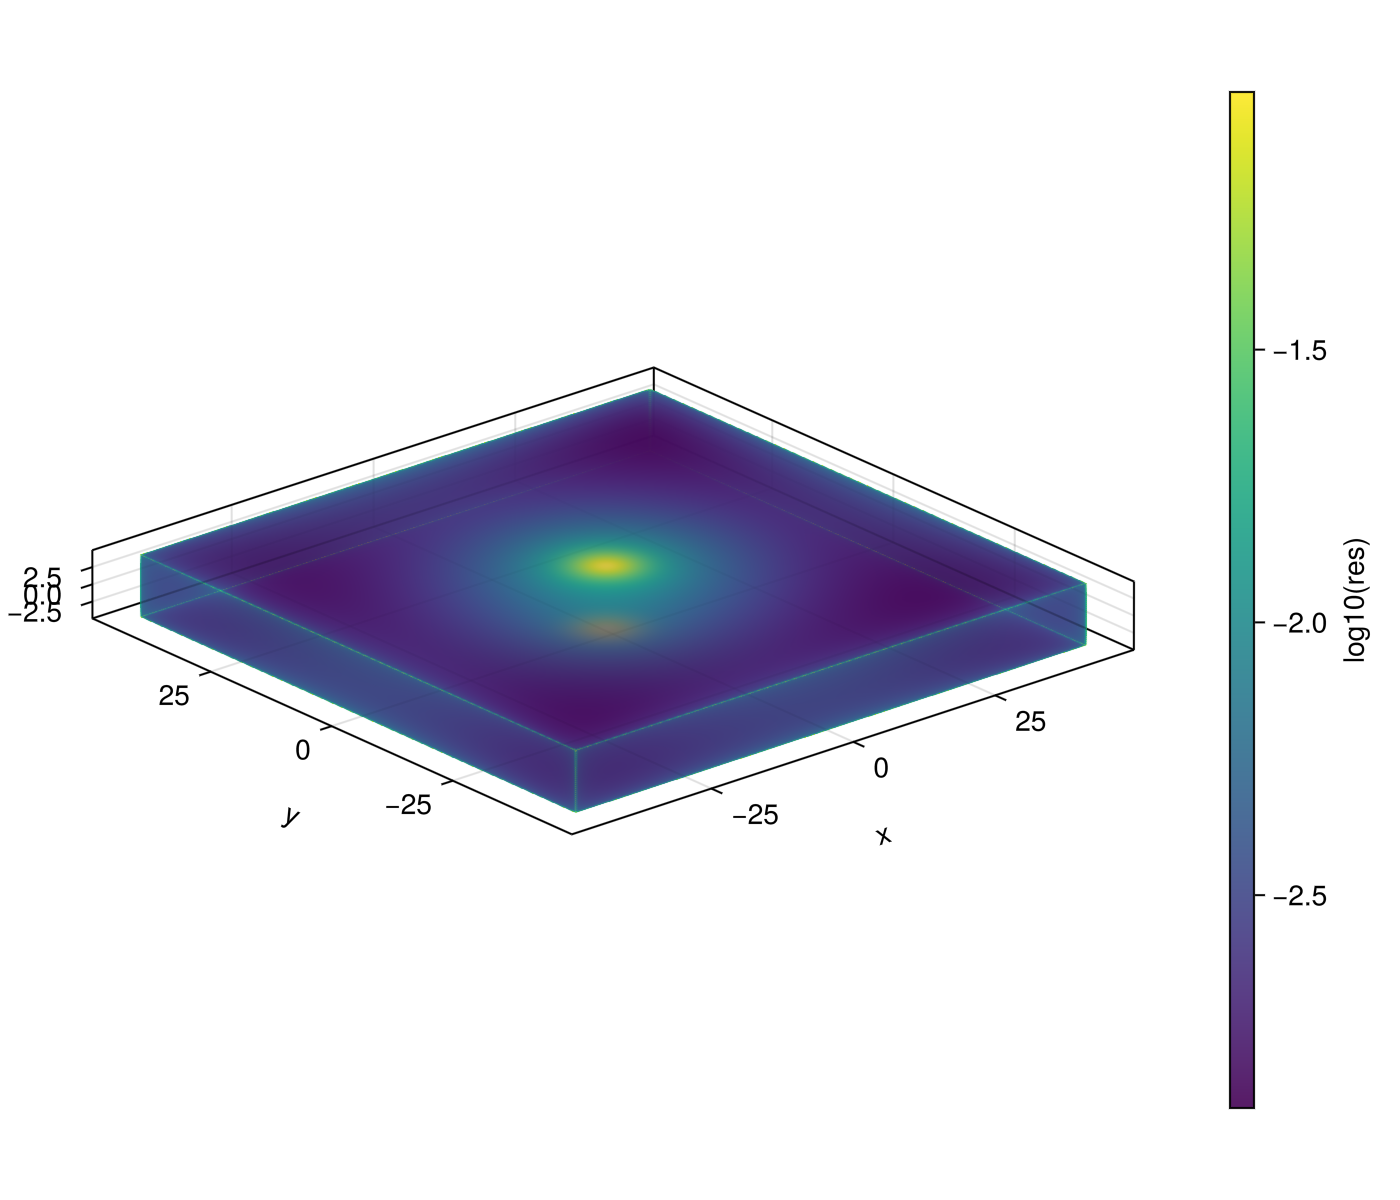
\includegraphics[width=\linewidth]{../codes/viz/figs/graphene_orbital_solution.png}
    \end{subfigure}
    \caption{RHS (left) and solution (right) of Eq.~\eqref{eq:sl_equation}.}
    \label{fig:rhs_solution}
\end{figure}

\FloatBarrier

Finally, with the discretized reprensentation of the surface charge density $\sigma(x)$, which is equal to a panel-wise polynomial, we can evaluate the potential at any point in the domain.
To validate the solver, we do a self convergence test by evaluating the potential at a set of fixed points with different order of quadrature and edge refinements, as shown in Fig.~\ref{fig:convergence}.

\begin{figure}
    \centering
    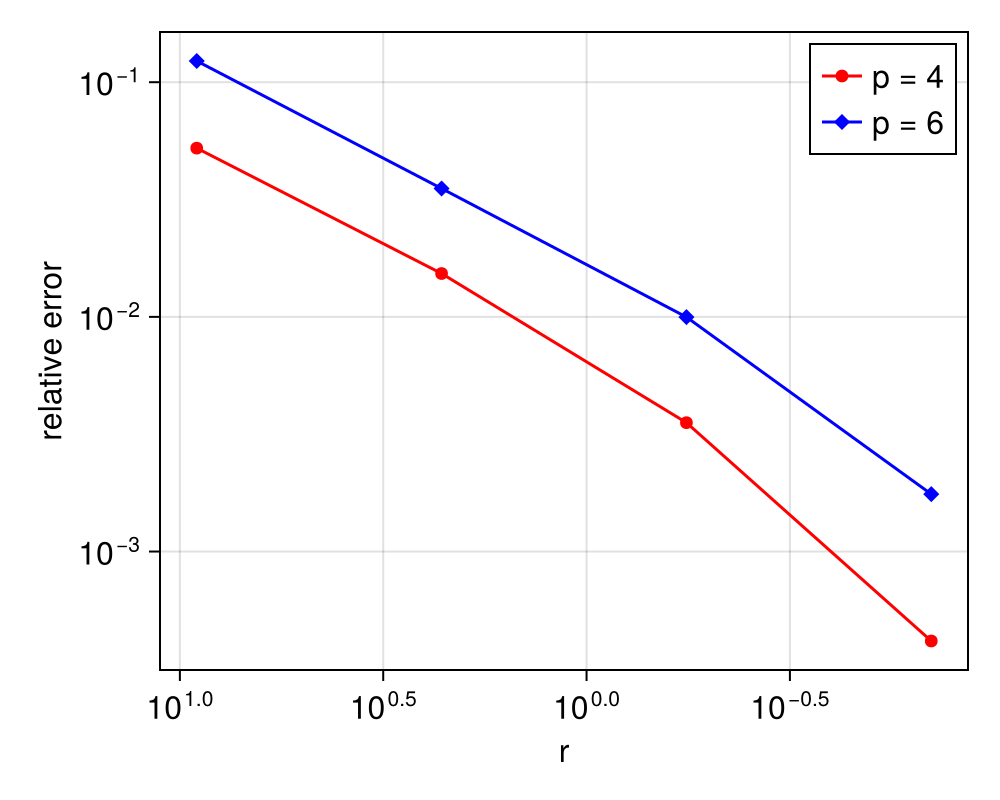
\includegraphics[width = 0.5\linewidth]{../codes/volume_source/figs/orbital_source_convergence.png}
    \caption{Convergence of the potential at fixed points with different order of quadrature and edge refinements.}
    \label{fig:convergence}
\end{figure}


% \bibliographystyle{apsrev}
\bibliography{ref}

\end{document}